\subsection{Verification of the interface reconstruction}

For structured meshes, a standard approach to computing the error of the
interface reconstruction algorithm (i.e.\ reconstruction error) resorts to
computing the volume that lies between the piecewise planar reconstructed
interface geometry and an analytical function representing the true interface
(e.g.\ the surface of a sphere).  This \emph {integration approach} requires
sub-integration for each cell.  Hence, it is not straightforward to modify the
algorithm in order to support arbitrary cell shapes.  

On arbitrary unstructured meshes, in order to achieve a single layer of
interface cells for a pre-processed volume fraction field, we have adopted the
approach by \citet{AhnShashkov2009} that involves intersecting two unstructured
meshes: the \emph{base mesh} and the \emph{tool mesh}. The \emph{base mesh} is
the mesh used to discretise the flow domain, and the \emph{tool mesh} is used
as a tool for cutting the \emph{base mesh} in order to set the volume fraction
field. This preprocessing approach of intersecting meshes allows for
preprocessing of arbitrarily complex volume fraction fields. Since the tool
mesh is unstructured, it may be used to discretize the complex input geometry.
Moreover, local refinement can easily be applied near boundaries that are used
to describe the fluid interface: this significantly reduces the computational
time of the preprocessing. The quality of the tool mesh is of virtually no
importance, since it is only use to set the initial volume fraction fields

In order to compute the reconstruction error on meshes with arbitrary cell
shapes, the reconstruction error is defined in each cell as the \emph{volume of
symmetric difference} ($E_{vsd}$) between the reconstructed geometry
(\emph{interface polyhedron}) and the true geometry. The true interface
geometry is represented by a subset of cells of a tool mesh, i.e.\ a set of
tool mesh boundary faces represent the true discrete interface geometry. 

\begin{figure}
   \centering
   %\def\svgwidth{\columnwidth}
   \def\svgwidth{0.6\columnwidth}
   {\footnotesize
       \input{figures/volumeOfSymmetricDifferenceActual.pdf-tex}
   }
   \caption{Volume of symmetric difference reconstruction error}
   \label{fig:volSymmDiff}
\end{figure}

The computation of the reconstruction error for a true interface geometry
defined by the tool mesh is performed cell-wise. Error calculation is
schematically described in two dimensions in Figure \ref{fig:volSymmDiff}. Each
mixed cell of the base mesh (dashed line) is intersected with a set of
polyhedrons of the tool mesh (green line). Each tool mesh polyhedron is then
clipped by the base mesh cell (black line). The reconstruction error (red
color) is separated into two contributions: \emph{positive half-space error}
($E_{vsd}^+$) and \emph{negative half-space error} ($E_{vsd}^-$), based on the
location of the error geometry with respect to the interface plane.

The set of tool mesh polyhedra is separated into two subsets based on the
interface plane orientation. The negative half-space error is the volume of
symmetric difference that lies in the negative closed half-space defined by the
interface plane. It is computed as an intersection between the set of the tool
mesh polyhedra clipped by the cell ($I_c$) and the negative half-space
($H(\vec{n})^-$), defined by the interface plane:
%
\begin{equation}
        E_{vsd}^{-} = || H(\vec{n})^- \cap I_{c} ||. 
\end{equation}
%
The positive half-space error is calculated as the algebraic difference between
the volume of the reconstructed (PLIC) polyhedron ($R_c$, blue line) and the
sum of the volumes of the clipped tool mesh polyhedra (black line): 
%
\begin{equation}
        E_{vsd}^+ = || R_c || - ||H(\vec{n})^+ \cap I_c||. 
\end{equation}
%
The total reconstruction error is computed as the sum of the positive
half-space error and the negative half-space error: 
%
\begin{equation}
        E_{vsd} = E_{vsd}^- + E_{vsd}^+.
\end{equation}
%
Note that when the \emph{integration approach} is used to determine the
reconstruction error the size of the sub-grid integration intervals will
determine the accuracy of the computed error (\cite{Aulisa2007}). The
\emph{mesh intersection approach} requires that the mesh density of the tool
mesh to be high enough in order to accurately describe the true interface
geometry. This is both visually observed and quantified for all validation
cases.   

\subsubsection{Reconstruction of a sphere} 

In this section the reconstruction results for a spherical interface on an
unstructured hexahedral, tetrahedral and polyhedral mesh are presented.  

%\begin{figure}
%   \centering
%      \begin{tikzpicture}
%         \begin{loglogaxis}[
%            %title={Reconstruction error: hexahedral mesh, sphere, NAG gradient},
%            xlabel=Volume numbers of the base meshes,
%            ylabel=Volume of symmetric difference, 
%            xtick=data,
%            grid=both,
%            xticklabels={$4^3$, $8^3$, $16^3$, $32^3$},
%            label style={font=\footnotesize}, tick label style={font=\footnotesize},
%            legend style={font=\footnotesize},
%            xmin=0, xmax=40000, 
%            ymin=1e-04, ymax=0.1]
%            \addplot table [x index=0, y index=1] {./figures/volSurfaceGauss-error.dat};
%            \addplot table [x index=0, y index=2] {./figures/volSurfaceGauss-error.dat};
%            \addplot table [x index=0, y index=3] {./figures/volSurfaceGauss-error.dat};
%             \legend{coarse, fine, very fine};
%         \end{loglogaxis}
%      \end{tikzpicture}
%    \caption{Reconstruction error for a sphere using the NAG gradient, on an unstructured hexahedral mesh} 
%    \label{fig:recError:sphere:NAG}
%\end{figure}
\begin{figure}
	\centering
		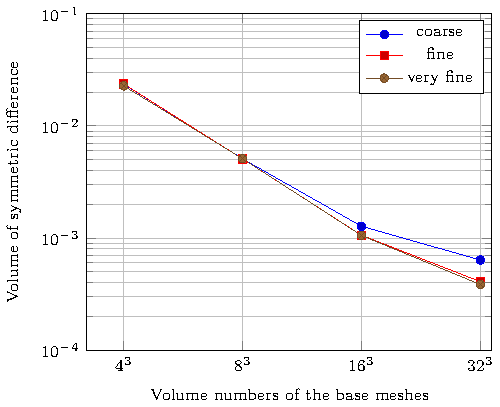
\includegraphics{./MaricMarschallBothe-voFoamAlgorithm-figure0.pdf}
    \caption{Reconstruction error for a sphere using the NAG gradient, on an unstructured hexahedral mesh} 
    \label{fig:recError:sphere:NAG}
\end{figure}


%\begin{figure}
%   \centering
%      \begin{tikzpicture}
%         \begin{loglogaxis}[
%            %title={Reconstruction error: hexahedral mesh, sphere, generalized LSQ gradient},
%            xlabel=Volume numbers of the base meshes, 
%            ylabel=Volume of symmetric difference, 
%            xtick=data,
%            grid=both,
%            xticklabels={$4^3$, $8^3$, $16^3$, $32^3$},
%            label style={font=\footnotesize}, tick label style={font=\footnotesize},
%            legend style={font=\footnotesize},
%            xmin=0, xmax=40000, 
%            ymin=1e-04, ymax=0.1]
%            \addplot table [x index=0, y index=1, ] {./figures/generalizedLsq-error.dat};
%            \addplot table [x index=0, y index=2] {./figures/generalizedLsq-error.dat};
%            \addplot table [x index=0, y index=3] {./figures/generalizedLsq-error.dat};
%             %\legend{coarse, fine, fineGauss,  very fine};
%             \legend{coarse, fine, very fine};
%         \end{loglogaxis}
%      \end{tikzpicture}
%
%    \caption{Reconstruction error for a sphere using the generalized LSQ gradient, on an unstructured hexahedral mesh}
%    \label{fig:recError:sphere:generalizedLsq}
%\end{figure}
\begin{figure}
	\centering
		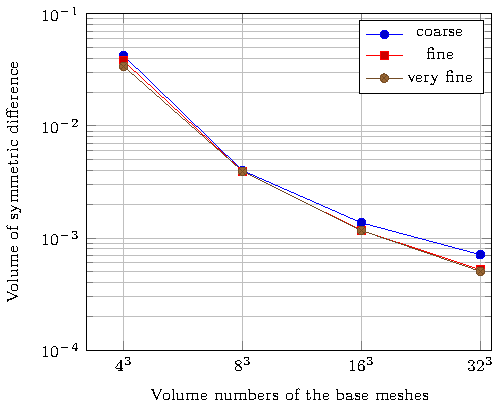
\includegraphics{./MaricMarschallBothe-voFoamAlgorithm-figure1.pdf}
    \caption{Reconstruction error for a sphere using the generalized LSQ gradient, on an unstructured hexahedral mesh}
    \label{fig:recError:sphere:generalizedLsq}
\end{figure}

Figures \ref{fig:recError:sphere:NAG} and
\ref{fig:recError:sphere:generalizedLsq} show the convergence diagrams of the
volume of symmetric difference reconstruction error on a box domain of
dimensions $[0,1]^3$ which is discretized with an \emph{unstructured hexahedral
mesh}. Although the discretization results in cuboid finite volumes, the mesh
connectivity is still unstructured. The first order Youngs algorithm exhibits
the behavior as described by \cite{AhnShashkovMultiMaterialRec2007}: on coarse
meshes the order of convergence of the error is higher and as the base
mesh density increases, the order reduces to around one. For the fine
tool mesh, the order of convergence as described by \cite{Aulisa2007} is
$2.22$ for the coarsest base mesh and $1.37$ for the finest base
mesh. 

\begin{figure}
   \begin{subfigure}[b]{0.45\columnwidth}
       \centering
       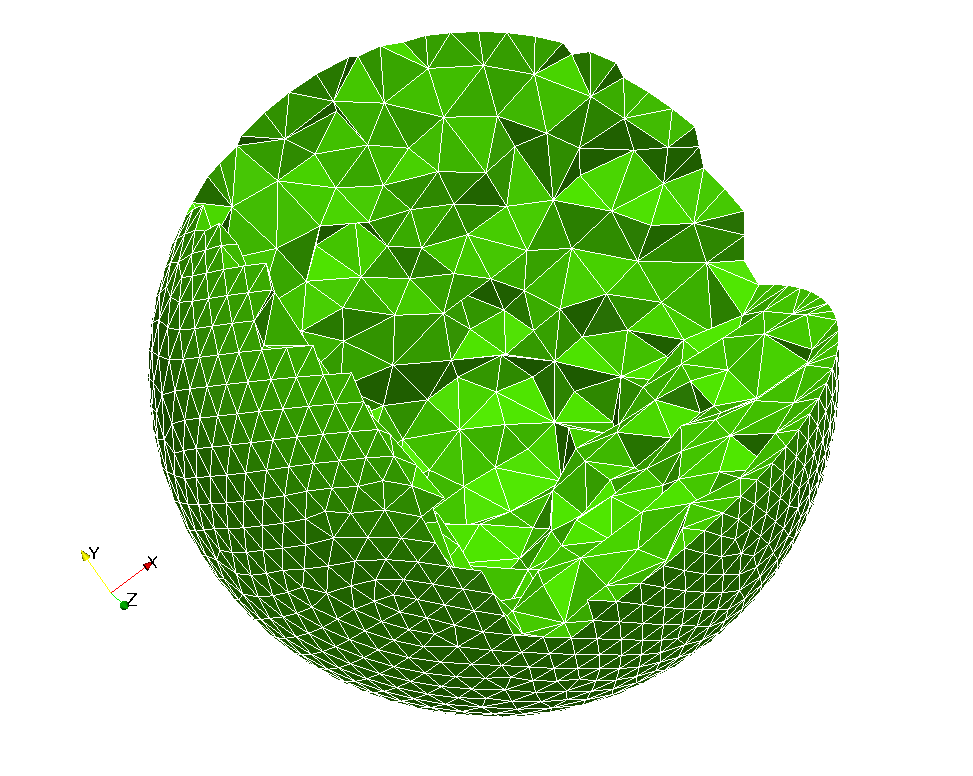
\includegraphics[width=\columnwidth]{figures/sphereFineMeshRefined.png}
       \label{fig:mesh:sphereFine:unrefined}
       \caption{Unrefined tool mesh}
   \end{subfigure}
   \begin{subfigure}[b]{0.45\columnwidth}
       \centering
       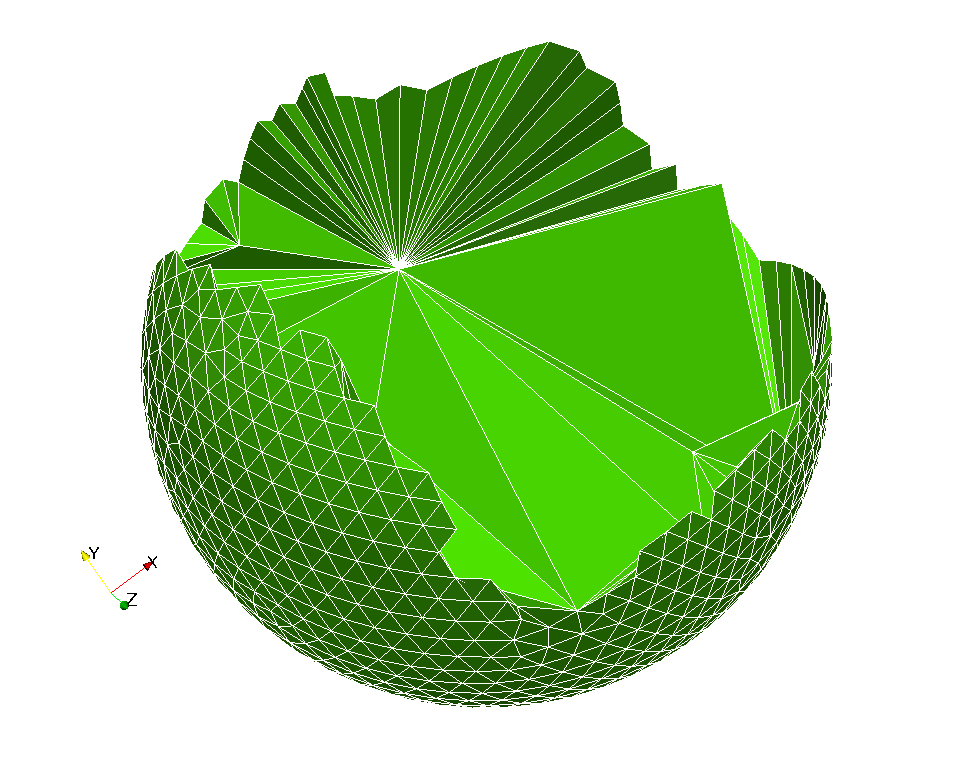
\includegraphics[width=\columnwidth]{figures/sphereFineMesh.png}
       \caption{Refined tool mesh}
       \label{fig:mesh:sphereFine:refined}
   \end{subfigure}

    \caption{Tool meshes of a spherical interface}
    \label{fig:mesh:sphereFine}
    \label{fig:mesh:sphereFine:unrefinedRefined}
\end{figure}

Different mesh densities were tested for a spherical tool mesh. The
local refinement of the tool mesh near the interface makes the
total number of cells not important rather the number of faces used to approximate
the spherical surface is central. Figure \ref{fig:mesh:sphereFine} shows two \emph{tool
meshes} of a sphere, each with the same number of face elements, but different
number of volumes. Both meshes are cut such that the inner mesh is visible: the
refined mesh has much less volumes, and both meshes describe the spherical
surface with the same mesh density. The tool mesh does not need to be of
high quality since it is not a part of the solution process, i.e. it is used
only for the preprocessing of the volume fraction field. Figure
\ref{fig:recError:sphere:unrefinedRefined} shows the convergence for the
reconstructed spherical interface on an unstructured hexahedral mesh with two
sphere tool meshes, namely a refined sphere, and an unrefined sphere (cp.\ 
Figure \ref{fig:mesh:sphereFine:unrefinedRefined}). 

%\begin{figure}
%   \centering
%      \begin{tikzpicture}
%         \begin{loglogaxis}[
%            %title={Reconstruction error of the refined/unrefined sphere tool mesh},
%            xlabel=Volume numbers of the base meshes,
%            ylabel=Volume of symmetric difference, 
%            xtick=data,
%            grid=both,
%            xticklabels={$4^3$, $8^3$, $16^3$, $32^3$},
%            label style={font=\footnotesize}, tick label style={font=\footnotesize},
%            legend style={font=\footnotesize},
%            xmin=0, xmax=40000, 
%            ymin=1e-04, ymax=0.1]
%            \addplot table [x index=0, y index=2] {./figures/volSurfaceGauss-error.dat};
%            \addplot table [x index=0, y index=1] {./figures/volSurfaceGauss-error-refined.dat};
%            \addplot table [x index=0, y index=2] {./figures/generalizedLsq-error.dat};
%            \addplot table [x index=0, y index=1] {./figures/generalizedLsq-error-refined.dat};
%            \legend{unrefined NAG, refined NAG, unrefined LSQ, refined LSQ};
%         \end{loglogaxis}
%      \end{tikzpicture}
%    \caption{Comparison of the reconstruction error convergence for the refined and unrefined tool mesh for a sphere}
%    \label{fig:recError:sphere:unrefinedRefined}
%\end{figure}
\begin{figure}
	\centering
		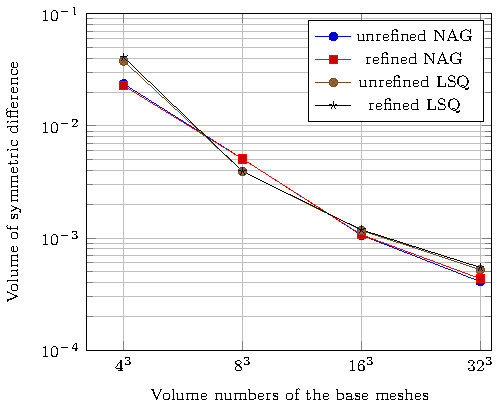
\includegraphics{./MaricMarschallBothe-voFoamAlgorithm-figure2.pdf}
    \caption{Comparison of the reconstruction error convergence for the refined and unrefined tool mesh for a sphere}
    \label{fig:recError:sphere:unrefinedRefined}
\end{figure}

For the mesh convergence study we have used spheres discretized with $956$,
$3786$ and $16462$ faces\footnote{The meshes were created with the \emph{open
source} application \emph{SalomeCAD}. They can be easily re-created using the
multiplication of the default parameters for the maximal edge length provided
by the NETGEN-1D-2D-3D algorithm by factors: $2$, $4$ and $8$.}. The surface
mesh densities of the sphere correspond to the case labels \emph{coarse},
\emph{fine} and \emph{very fine} used in the Figures
\ref{fig:recError:sphere:NAG} and \ref{fig:recError:sphere:generalizedLsq}.
%Although the sphere tool meshes show similar convergence behavior, the
The \emph{fine} sphere mesh is chosen for further results comparison.

\begin{figure}
   {\footnotesize
   \begin{center}
   \begin{subfigure}[]{0.45\columnwidth}
       \centering
       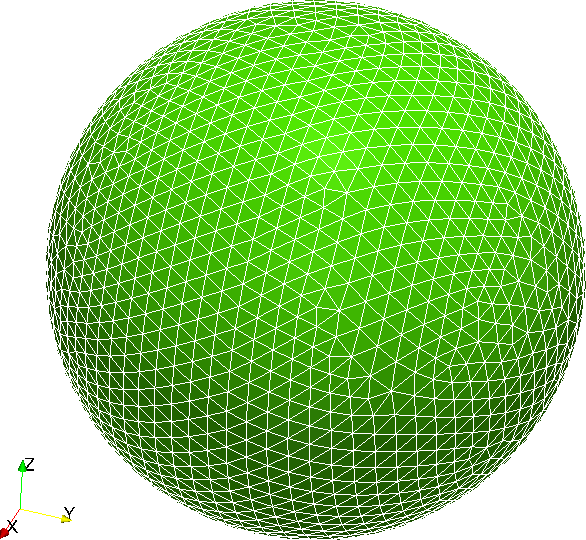
\includegraphics[width=0.6\columnwidth]{figures/sphereFineComplete.png}
       \caption{Sphere tool mesh (\emph{fine} case)}
       \label{fig:recResults:sphereMesh}
   \end{subfigure}
   \end{center}
   \begin{subfigure}[b]{0.45\columnwidth}
       \centering
       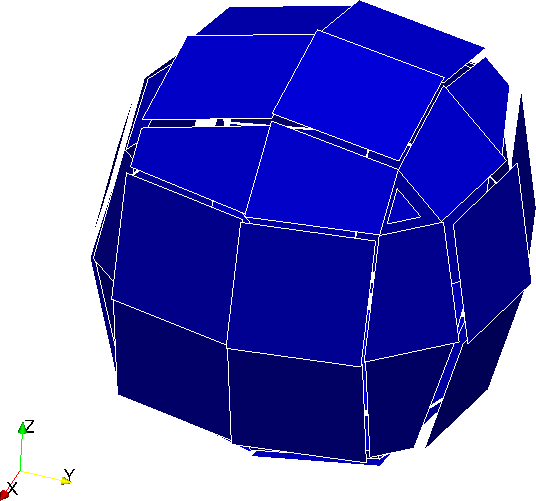
\includegraphics[width=0.6\columnwidth]{figures/sphereFine-gauss-004.png}
       %\caption{Reconstructed sphere: NAG gradient, mesh density is $4^3$}
       %\label{fig:mesh:sphereFine:unrefined}
   \end{subfigure}
   \begin{subfigure}[b]{0.45\columnwidth}
       \centering
       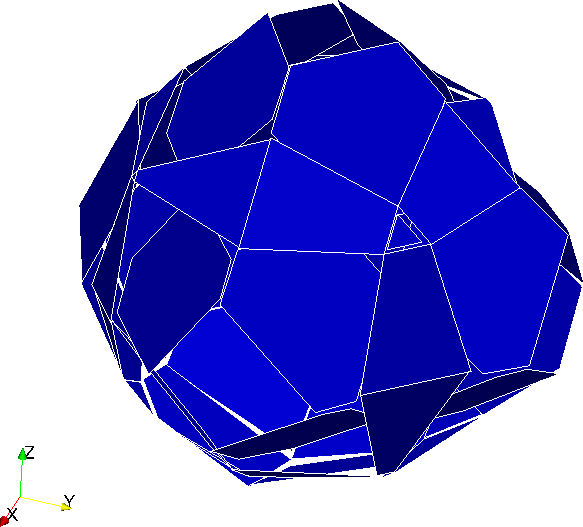
\includegraphics[width=0.6\columnwidth]{figures/sphereFine-LSQ-004.png}
       %\label{fig:mesh:sphereFine:refined}
       %\caption{Reconstructed sphere: generalized LSQ gradient, mesh density is $4^3$}
   \end{subfigure}

   \begin{subfigure}[b]{0.45\columnwidth}
       \centering
       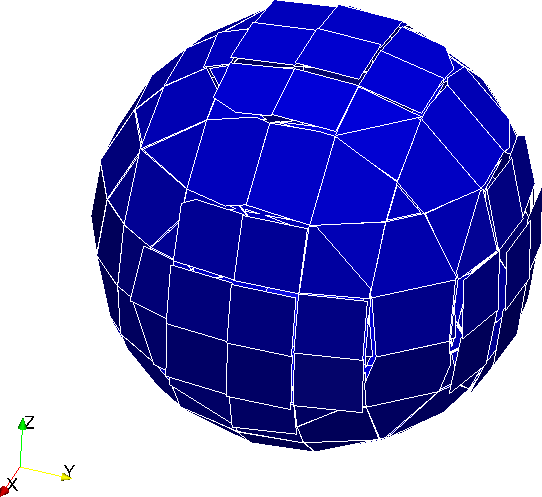
\includegraphics[width=0.6\columnwidth]{figures/sphereFine-gauss-008.png}
       %\caption{Reconstructed sphere: NAG gradient, mesh density is $8^3$}
       %\label{fig:mesh:sphereFine:unrefined}
   \end{subfigure}
   \begin{subfigure}[b]{0.45\columnwidth}
       \centering
       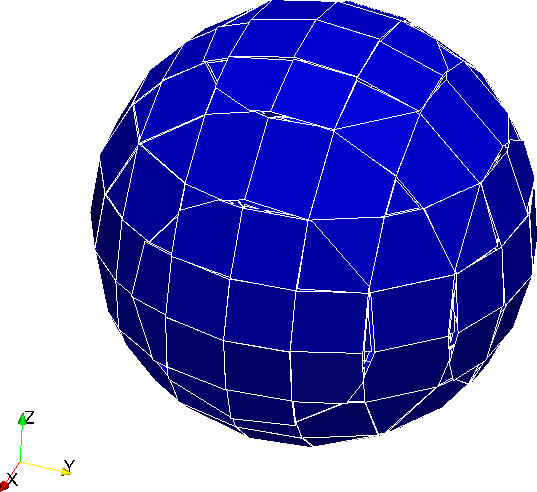
\includegraphics[width=0.6\columnwidth]{figures/sphereFine-LSQ-008.png}
       %\label{fig:mesh:sphereFine:refined}
       %\caption{Reconstructed sphere: generalized LSQ gradient, mesh density is $8^3$}
   \end{subfigure}

   \begin{subfigure}[b]{0.45\columnwidth}
       \centering
       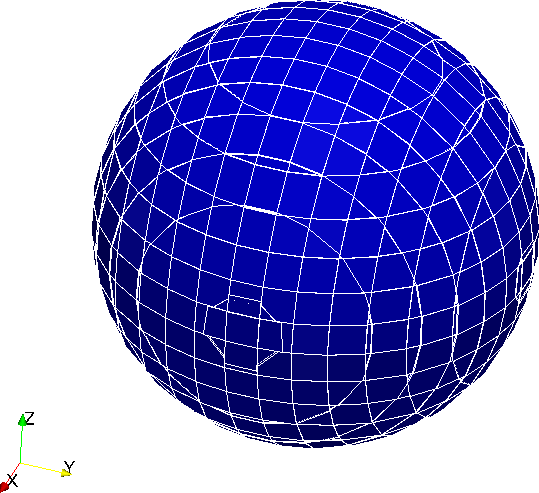
\includegraphics[width=0.6\columnwidth]{figures/sphereFine-gauss-016.png}
       %\caption{Reconstructed sphere: NAG gradient, mesh density is $16^3$}
       %\label{fig:mesh:sphereFine:unrefined}
   \end{subfigure}
   \begin{subfigure}[b]{0.45\columnwidth}
       \centering
       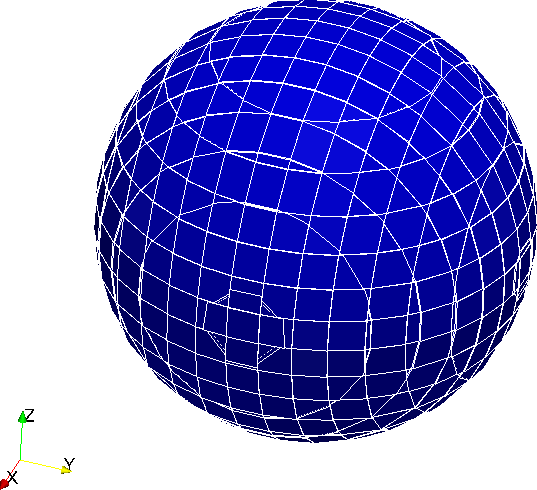
\includegraphics[width=0.6\columnwidth]{figures/sphereFine-LSQ-016.png}
       %\label{fig:mesh:sphereFine:refined}
       %\caption{Reconstructed sphere: generalized LSQ gradient, mesh density is $16^3$}
   \end{subfigure}

   \begin{subfigure}[b]{0.45\columnwidth}
       \centering
       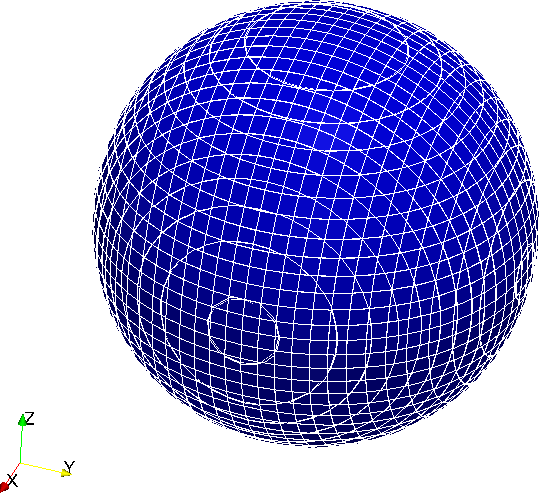
\includegraphics[width=0.6\columnwidth]{figures/sphereFine-gauss-032.png}
       %\caption{Reconstructed sphere: NAG gradient, mesh density is $32^3$}
       %\label{fig:mesh:sphereFine:unrefined}
       \caption{NAG gradient}
   \end{subfigure}
   \begin{subfigure}[b]{0.45\columnwidth}
       \centering
       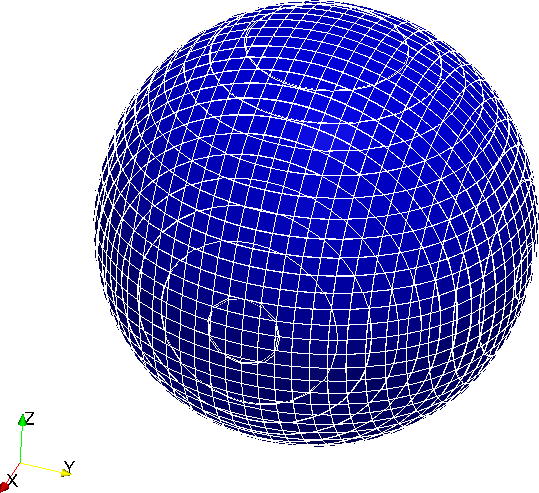
\includegraphics[width=0.6\columnwidth]{figures/sphereFine-LSQ-032.png}
       %\label{fig:mesh:sphereFine:refined}
       %\caption{Reconstructed sphere: generalized LSQ gradient, mesh density is $32^3$}
       \caption{generalized LSQ gradient}
   \end{subfigure}

    \caption{Reconstructed spherical interface on an unstructured hexahedral
mesh. Interfaces are reconstructed on base meshes with densities: $4^3$, $8^3$,
$16^3$ and $32^3$} 

    \label{fig:recResults:comparison}
   }
\end{figure}

Figure \ref{fig:recResults:comparison} shows the input mesh for the sphere
(\emph{fine} case) and the comparison of the corresponding reconstructed
interfaces using both the NAG  gradient and the generalized LSQ gradient on
unstructured hexahedral meshes. The NAG gradient shows better results on the
coarsest hexahedral mesh in the volume of symmetric difference error.  This can
be seen when the absolute values are compared for the coarsest \emph{base
meshes} shown in Figures \ref{fig:recError:sphere:NAG} and
\ref{fig:recError:sphere:generalizedLsq}. Also, the visual appearance of the
interface geometry on the coarsest mesh is clearly better when the NAG gradient
is applied on an unstructured hexahedral mesh, as shown in Figure
\ref{fig:recResults:comparison}.

\begin{figure}
   {\footnotesize
   \begin{center}
   \begin{subfigure}[]{0.45\columnwidth}
       \centering
       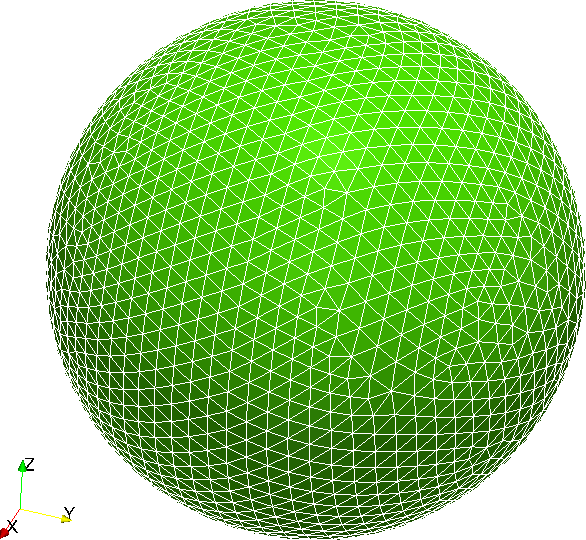
\includegraphics[width=0.54\columnwidth]{figures/sphereFineComplete.png}
       \caption{Sphere tool mesh (\emph{fine} case)}
       \label{fig:recResults:sphereMeshTet}
   \end{subfigure}
   \end{center}

   \begin{subfigure}[b]{0.45\columnwidth}
       \centering
       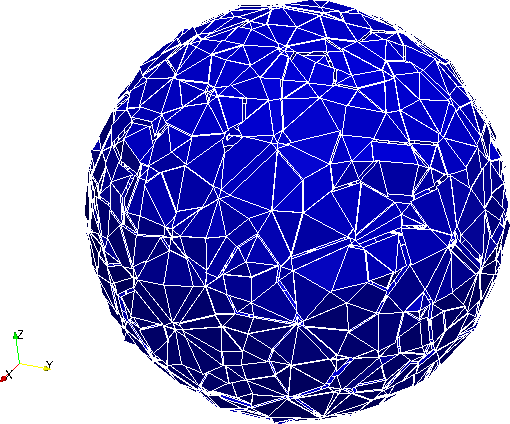
\includegraphics[width=0.6\columnwidth]{figures/sphereFineTet-gauss.png}
       \caption{NAG gradient} 
       %\label{fig:mesh:sphereFine:unrefined}
   \end{subfigure}
   \begin{subfigure}[b]{0.45\columnwidth}
       \centering
       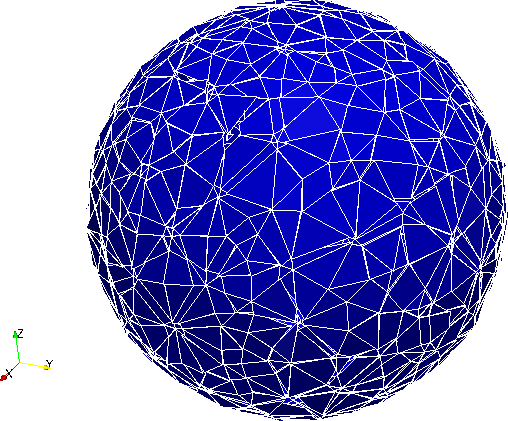
\includegraphics[width=0.6\columnwidth]{figures/sphereFineTet-LSQ.png}
       %\label{fig:mesh:sphereFine:refined}
       \caption{Generalized LSQ gradient}
   \end{subfigure}

    \caption{Reconstructed spherical interface on an unstructured tetrahedral 
mesh. Interfaces are reconstructed on a base mesh with $8774$ volumes}
    \label{fig:recResults:comparisonTet}
   }
\end{figure}

% Convergence diagram for the tetrahedral mesh. Both gradients. 
%\begin{figure}
%   \centering
%      \begin{tikzpicture}
%         \begin{loglogaxis}[
%            %title={Reconstruction error: sphere, unstructured mesh},
%            xlabel=Density of the base mesh,
%            ylabel=Volume of symmetric difference, 
%            %xtick=data,
%            grid=both,
%            %xticklabels={"857", "2168", "8774", "20263"},
%            label style={font=\footnotesize}, tick label style={font=\footnotesize},
%            legend style={font=\footnotesize},
%            xmin=0, xmax=30000, 
%            ymin=1e-04, ymax=1e-01]
%            \addplot table [x index=0, y index=1] {./figures/volSurfaceGauss-error-tetra.dat};
%            \addplot table [x index=0, y index=1] {./figures/generalizedLsq-error-tetra.dat};
%
%            \legend{NAG, generalized LSQ};
%         \end{loglogaxis}
%      \end{tikzpicture}
%
%    \caption{Reconstruction error for a sphere on a tetrahedral mesh with following numbers of volumes: 857, 2168, 8774, 20263}
%    \label{fig:recError:sphere:tetra}
%\end{figure}
\begin{figure}
	\centering
		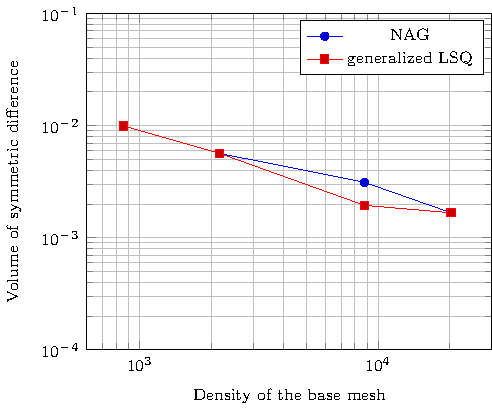
\includegraphics{./MaricMarschallBothe-voFoamAlgorithm-figure3.pdf}
    \caption{Reconstruction error for a sphere on a tetrahedral mesh with following numbers of volumes: 857, 2168, 8774, 20263}
    \label{fig:recError:sphere:tetra}
\end{figure}

Figure \ref{fig:recResults:comparisonTet} shows the reconstructed spherical
interfaces on a tetrahedral mesh. For this case the error magnitude is lower
when the NAG gradient is applied. Interface polygons on a tetrahedral mesh are
significantly disconnected, especially around the reconstruction points where
multiple tetrahedra meet in a mesh vertex. Around those points the volume
fraction values will be either very small ($\alpha_1 \approx 0$) or very large
($\alpha_1 \approx 1$) in which cases even the smallest perturbation in the
orientation of the interface normal causes significant disconnection of the
interface polygons. 

Figure \ref{fig:recError:sphere:tetra} shows the behavior of the interface
reconstruction error on an \emph{unstructured tetrahedral mesh}. The evaluation
of the reconstruction error is done for both the NAG gradient and the
generalized LSQ gradient. Both gradients show similar behavior of the error
magnitude with respect to the increase of the mesh density. On a tetrahedral
mesh the evaluation of the error convergence is not possible, because of its
irregular nature. Still, the diagram shown in Figure
\ref{fig:recError:sphere:tetra} shows that the magnitude of the reconstruction
error does not decrease as fast as on the unstructured hexahedral mesh. This
fact brings us to conclusion that the unstructured hexahedral mesh makes a
better choice for domain discretization for our geometrical VoF method. 

A polyhedral mesh provides direct connectivity via finite volume faces to all
surrounding cells which makes the gradient calculation more exact and
straightforward since it relies on the connectivity which is already present
and involves all available cell neighbors. However, the quality of the
polyhedral mesh will rely on the way it is created, which is usually done by
agglomerating tetrahedral cells. When tetrahedral cells are agglomerated to
create polyhedra, severely non-convex cells with significant non-planarity of
faces, appear in the mesh if the original tetrahedral mesh is not produced with
the Delaunay algorithm. Severely non-convex cells introduce numerical errors
and are unusable together with the intersection algorithms used for the
geometrical VoF method.

To the best of our knowledge, a dynamic mesh refinement algorithm based
exclusively on polyhedral cells does not exist. Since we are interested in a
more accurate spatial resolution in the surrounding of a \emph{moving fluid
interface} (achieved by employing local dynamic AMR), the polyhedral mesh
results are shown only to prove the generality of the implemented geometrical
operations with respect to different cell shapes. % Figure
\ref{fig:recResults:comparisonPoly} shows the reconstruction of a spherical
interface on a polyhedral base mesh which is created by agglomerating the
tetrahedra of a mesh discretized using equal sized hexahedral cells. The
hexahedral cells are then decomposed, each into $24$ tetrahedrons, which are
then agglomerated into polyhedra to ensure the convexity of the cells. This
mesh is then a mixture of hexahedral and polyhedral cells which is clearly
visible in the reconstructed interfaces. 

The behavior of the reconstruction error shows that there is a significant
accuracy gain in reconstructing the interface on an unstructured hexahedral
mesh, compared to the unstructured tetrahedral mesh. This type of mesh supports
local dynamic AMR within the frame of the existing topological mesh operations
in OpenFOAM: hexahedral refinement of cells. Moreover, the automatic mesh
generation of unstructured hexahedral meshes is widely available (e.g. via the
\emph{snappyHexMesh} tool of the OpenFOAM library). Hence, the unstructured
hexahedral mesh presents a natural choice for the domain discretization of a
geometrical VoF method supporting local dynamic AMR.

\begin{figure}
   {\footnotesize
   \begin{center}
   \begin{subfigure}[]{0.5\columnwidth}
       \centering
       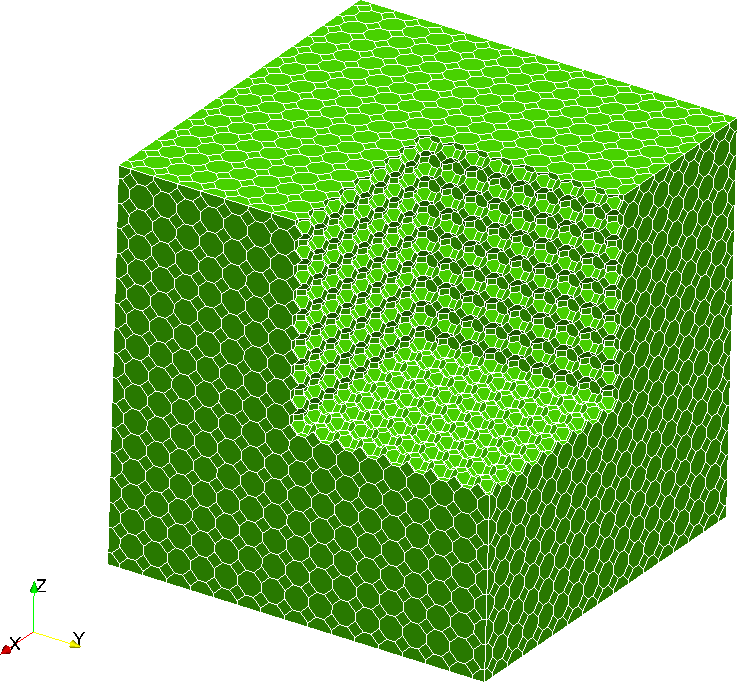
\includegraphics[width=0.9\columnwidth]{figures/mixedBasePolyMesh.png}
       \caption{Mixed polyhedral/hexahedral base mesh}
       \label{fig:recResults:sphereMeshPoly}
   \end{subfigure}
   \end{center}

   \begin{subfigure}[b]{0.45\columnwidth}
       \centering
       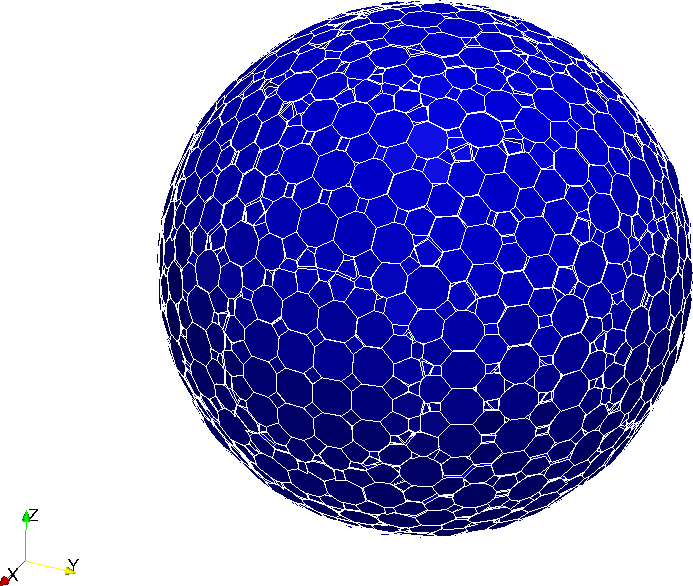
\includegraphics[width=0.6\columnwidth]{figures/sphereFine-gauss-poly.png}
       \caption{NAG gradient} 
       %\label{fig:mesh:sphereFine:unrefined}
   \end{subfigure}
   \begin{subfigure}[b]{0.45\columnwidth}
       \centering
       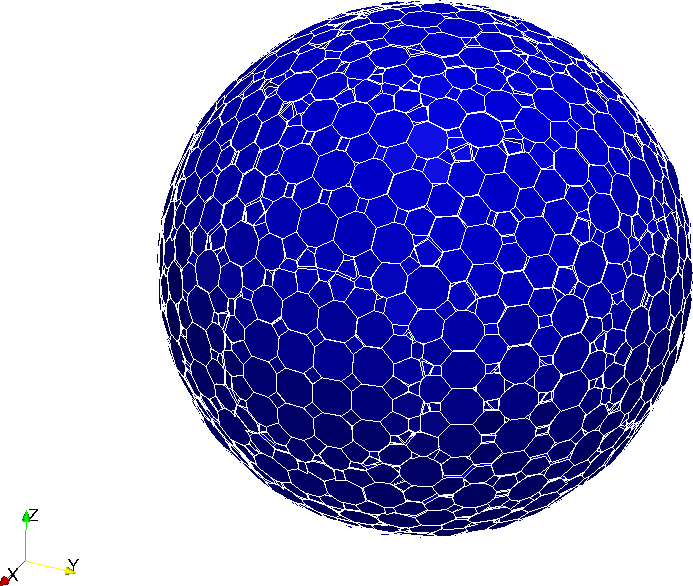
\includegraphics[width=0.6\columnwidth]{figures/sphereFine-LSQ-poly.png}
       %\label{fig:mesh:sphereFine:refined}
       \caption{Generalized LSQ gradient}
   \end{subfigure}

    \caption{Reconstructed spherical interface on a mixed polyhedral mesh with $22065$ cells} 

    \label{fig:recResults:comparisonPoly}
   }
\end{figure}



\subsection{Verification of the volume fraction advection}

In this section the results of the geometrical advection algorithm for standard
test cases are shown. Standard test cases are used to validate mass/volume
conservation, numerical boundedness of the volume fraction field i.e.
$\alpha_1 \in [0 + \epsilon,1 - \epsilon]$, where $\epsilon$ is the
reconstruction tolerance, geometrical stability of the interface as well as its
\emph{physically consistent motion}. A physically consistent motion of the
interface is a motion during which no \emph{artificial separation} is present
(e.g.  \emph{flotsam}/\emph{jetsam}), appearance of \emph{wisps} and
\emph{artificial deformation} of the interface are reduced to a minimum. 

\begin{description}
 \item Artificial separation of the interface involves large separated parts of the
fluid (flotsam and jetsam), as well as small changes in the volume fraction
field (wisps).Flotsam and jetsam are large parts of the interface that separate
during the advection artificially, as defined by \citet{NohWoodwardSLIC1976}.
Wisps are, usually very small, numerically artificial, interface polygons that
appear sporadically near the transported interface, as well as within the bulk.
In effect, this means that there is an additional layer of cells to the actual
interface cell layer, where the values of the volume fraction are either very
close to one ($\alpha \approx 1$) or to zero ($\alpha \approx 0$) for cells
that are not interface cells. Visualization of bulk wisps, as well as their
generation will depend on the reconstruction tolerance of the algorithm.
Reducing the reconstruction tolerance, will make the actual bulk wisp cell a
full cell, on account of introducing an error in mass conservation for this
cell. The presence of wisps in the bulk of the flow is due to the
non-divergence-free nature of the discrete flow field, which we counter in our
algorithm by introducing a narrow layer of cells where the advection takes
place. 

\item Artificial deformation of the interface is an interface motion which, although
resulting with a mass conservative volume fraction field bounded between $0$
and $1$, imposes an artificial change in the velocity with which the interface
is locally advected.  This error stems directly from the way the volumetric
phase flux is computed. 
\end{description}

The standard $E_g$ geometrical advection error is defined as follows
\citep{Aulisa2007}:
%
\begin{equation}
        E_g = \sum_c V_c (\alpha_c(t) - \alpha_c(t_0)),
        \label{eq:error:geom}
\end{equation}
%
where $c$ marks the cell of the volume $V_c$, $t$ marks the time value for
which the error is computed and $t_0$ marks the initial (reference) time value.
This error can only be applied for advection test cases for which the interface
configuration at time $t$ corresponds to the configuration at the initial time
$t_0$. For such cases, a periodical velocity field is used for advection.
Examples of such test cases are described by various authors and we have
used the following test cases to verify the geometrical advection algorithm:

\begin{compactitem}
   \item periodical translation along spatial diagonal,  
   \item rotation,  
   \item shear,  
   \item deformation. 
\end{compactitem} 

%At this point we would like to point out that the \emph{narrowing of the advection
%region was not applied} for the test cases, in order to test the mass
%conservation and numerical boundedness of the advection scheme even for the
%bulk flow.  

%The mass conservation error is defined as follows: 

%\begin{equation}
        %E_m (t) = add 
        %\label{eq:error:mass}
%\end{equation}

\subsubsection{Translation and rotation test}

Apart from a sharp interface representation within a single layer of cells, the
geometrical VoF method significantly reduces the artificial deformation of the
interface compared with algebraic VoF methods. Since there is a contribution to 
the volumetric phase flux coming from the point-cell neighbor cells (skew cell 
neighbors), the motion of the interface in this direction will not be artificially 
changed to a large extent. If the flux contributions stemming from the skew cell 
neighbors are completely neglected, as this is the case for algebraic advection 
schemes,  interface will be advected adhering to mass conservation, but the 
interface shape will be artificially changed to a large extent. 

The translation test case consists of a sphere of radius $0.15$, placed in the
center of a unit length box-domain with increasing uniform density, and it is
advected with Courant numbers: $0.1$, $0.5$ and $0.75$. The sphere is
translated along the spatial diagonal from the initial position to the two
orners of the box-domain and returned to initial position at the box center.
The overall distance traveled by the sphere in this test case is approximately 10
sphere diameters.  

\begin{figure}
   {\footnotesize
   \centering
   \begin{subfigure}[b]{0.49\columnwidth}
       \centering
       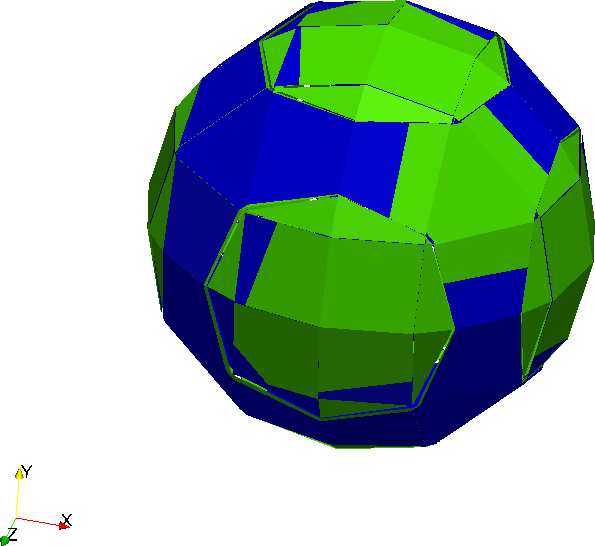
\includegraphics[width=\columnwidth]{figures/translation-hex-16-Co-05.png}
       \caption{Mesh with $16^3$ volumes} 
       %\label{fig:mesh:sphereFine:unrefined}
   \end{subfigure}
   \begin{subfigure}[b]{0.49\columnwidth}
       \centering
       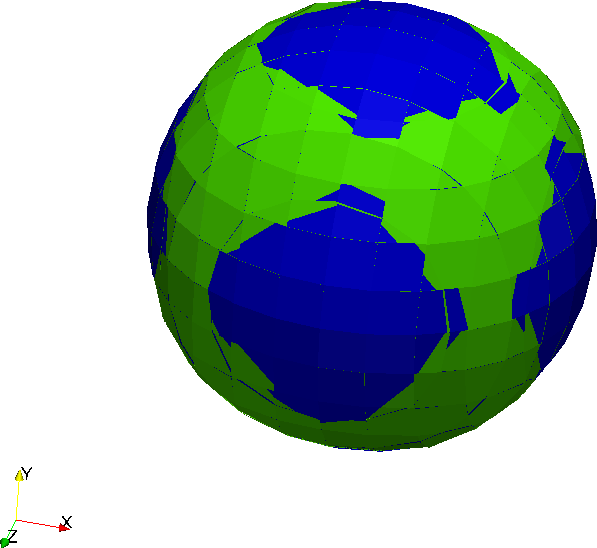
\includegraphics[width=\columnwidth]{figures/translation-hex-32-Co-05.png}
       %\label{fig:mesh:sphereFine:refined}
       \caption{Mesh with $32^3$ volumes}
   \end{subfigure}
\vspace{0.5cm}

   \begin{subfigure}[b]{0.49\columnwidth}
       \centering
       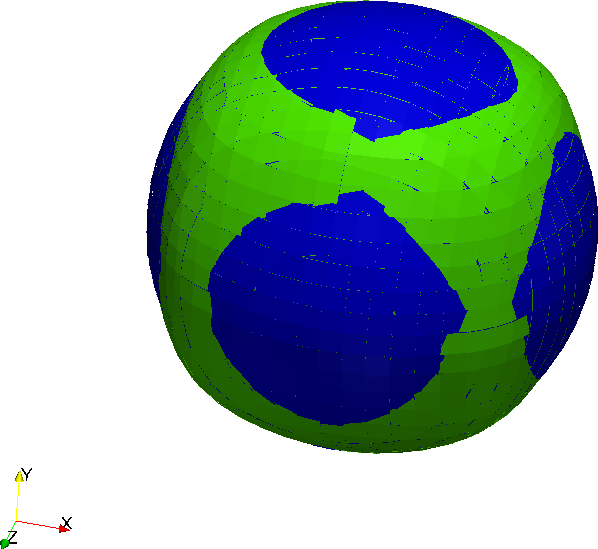
\includegraphics[width=\columnwidth]{figures/translation-hex-64-Co-05.png}
       \caption{Mesh with $64^3$ volumes}
       %\label{fig:mesh:sphereFine:unrefined}
   \end{subfigure}
   \begin{subfigure}[b]{0.49\columnwidth}
       \centering
       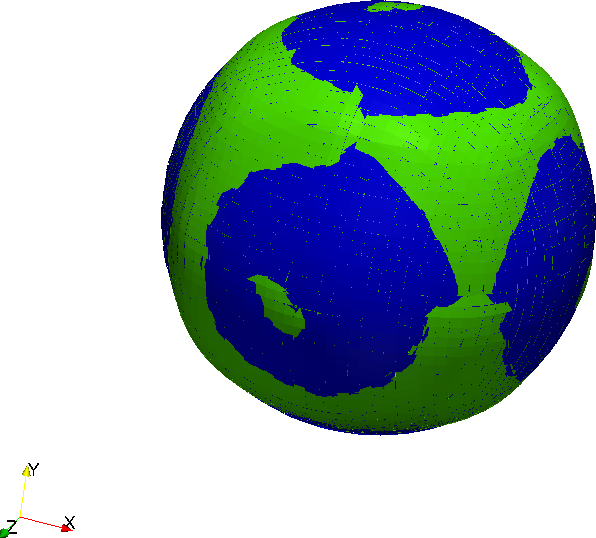
\includegraphics[width=\columnwidth]{figures/translation-hex-128-Co-05.png}
       %\label{fig:sphereFine:refined}
       \caption{Mesh with $128^3$ volumes}
   \end{subfigure}

    \caption{Visual comparison of the initial (blue) and the final sphere shape
(green) for mesh different densities of the \emph{skew advection} test}

    \label{fig:skew:initialFinal}
   }
\end{figure}

Figure \ref{fig:skew:initialFinal} shows a comparison between the final
position of the sphere and the initial sphere position for increasing mesh
density and the Courant number of $0.5$. For an advection directed along the
spatial diagonal, the images show that the flux calculation, although fully
un-split, involves a slight deformation of the interface the skew direction.
Table \ref{tab:errors:translation} shows the geometrical error ($E_g$) for the
skew-translation test case. The relative mass conservation error values are
near machine tolerance for the constant translation velocity field and are thus
omitted. 

\begin{table} 
\footnotesize
\centering 
\caption{Advection errors of the periodical translation test case} 
\label{tab:errors:translation} 
\begin{tabular}{c l c c c c c} 
       \toprule
       Number of volumes && $16^3$ & $32^3$ & $64^3$ & $128^3$ & \\ 
        \hline
        \hline
      Courant number &&&&&& \\
      0.1  $$ && 5.32128e-04 & 4.24662e-04  & 8.76037e-04 & 6.99539e-04 & \\ 
      0.5  $$ && 2.75337e-04 & 3.85527e-04  & 7.54332e-04 & 4.39392e-04 &\\ 
      0.75 $$ && 3.15498e-04 & 4.10146e-04  & 6.86752e-04 & 5.82132e-04 &\\ 
        \bottomrule
\end{tabular}
\end{table}

\begin{table} 
\footnotesize
    \centering 
    \caption{Advection errors for the rotation test case} 
    \label{tab:errors:rotation} 
    \begin{tabular}{c  c c c c c} 
          \toprule
          Number of volumes & $16^3$ & $32^3$ & $64^3$ & $128^3$ & \\ 
          \hline
          \hline
          $E_g$ & 8.32758e-04 &  3.18881e-04 & 1.45851e-04 & 1.11573e-04 & \\ 
          \bottomrule
    \end{tabular}
\end{table}

The rotation test case consists of a sphere with the radius of $0.15$ placed at
$(0.5, 0.75, 0.5)$ within a unit-length box domain as described by
\citet{jofreUnstructuredPLIC}. The sphere is rotated with a Courant number
value of  $0.5$ based on the maximal velocity used to advect the interface. The
final and initial positions of the sphere are compared. Table
\ref{tab:errors:rotation} shows the behavior of the advection error $E_g$  
with respect to the increase of mesh density for the rotation test case. Figure
\ref{fig:rotation:initialFinal} shows the visual comparison between the final
and initial interface shape for different densities of the mesh. The rotation
test case involves computing intersections with very thin and distorted flux
polyhedra, and for this purpose the rotation test cases with mesh densities of
$64^3$ and $128^3$ were run in parallel such that the process boundary plane
lies orthogonal to the velocity field. This test stresses the robustness and
accuracy of the geometrical advection algorithm even for extreme shapes of very
thin flux polyhedra. 

The visual difference between the initial sphere on the left process boundary
(blue) and the final sphere on the right process boundary (green) shown on the
Figure \ref{fig:rotation:initialFinal} is not noticeable. For the coarser
meshes of $32^3$ and $16^3$ volumes, the overlap shown on a single process
domain is insignificant, which is confirmed by absolute values of the $E_g$
error. The error convergence behaves as reported by other authors
\citep{HernandezLopezPart1Advection2008}: the error converges faster on coarser
meshes and the magnitude of order of convergence magnitude is near $1$, since
it is defined by the convergence order of the Young's reconstruction algorithm.  

\begin{figure}
   {\footnotesize
   \centering
   \begin{subfigure}[b]{0.49\columnwidth}
       \centering
       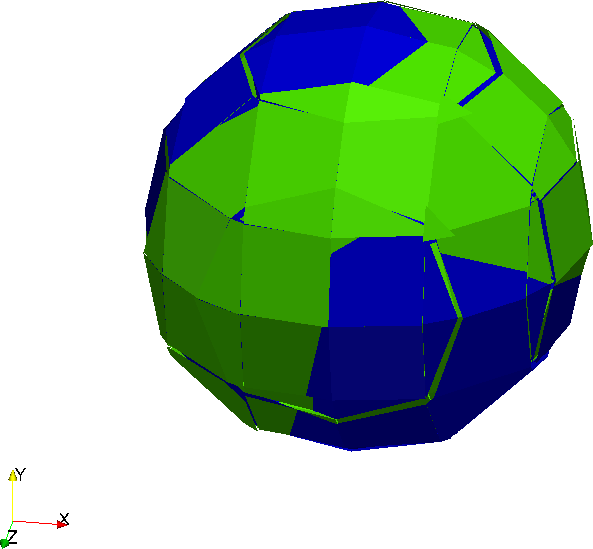
\includegraphics[width=\columnwidth]{figures/rotation-hex-16-Co-05.png}
       \caption{Mesh with $16^3$ volumes} 
       %\label{fig:mesh:sphereFine:unrefined}
   \end{subfigure}
   \begin{subfigure}[b]{0.49\columnwidth}
       \centering
       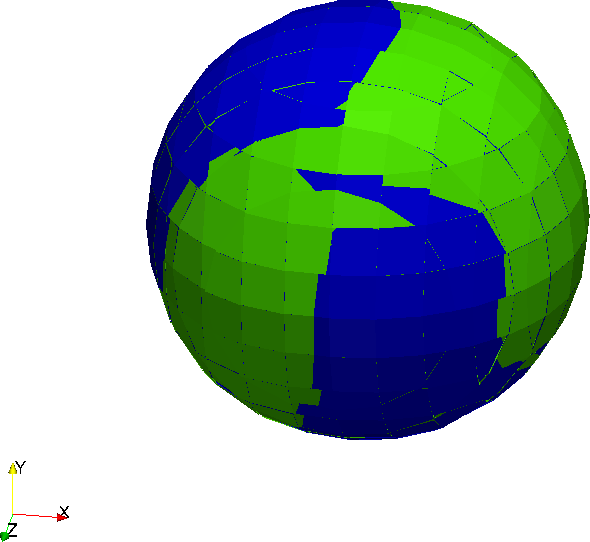
\includegraphics[width=\columnwidth]{figures/rotation-hex-32-Co-05.png}
       %\label{fig:mesh:sphereFine:refined}
       \caption{Mesh with $32^3$ volumes}
   \end{subfigure}

   \begin{subfigure}[b]{0.49\columnwidth}
       \centering
       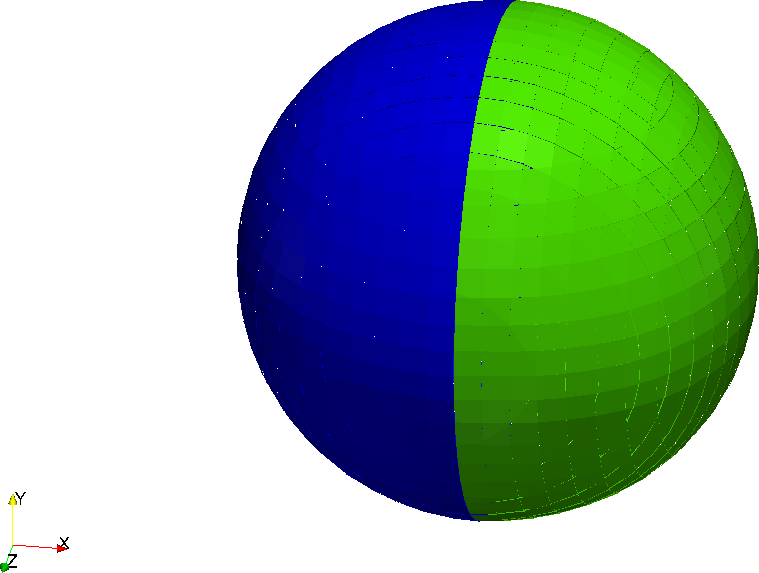
\includegraphics[width=\columnwidth]{figures/rotation-hex-64-Co-05.png}
       \caption{Mesh with $64^3$ volumes}
       %\label{fig:mesh:sphereFine:unrefined}
   \end{subfigure}
   \begin{subfigure}[b]{0.49\columnwidth}
       \centering
       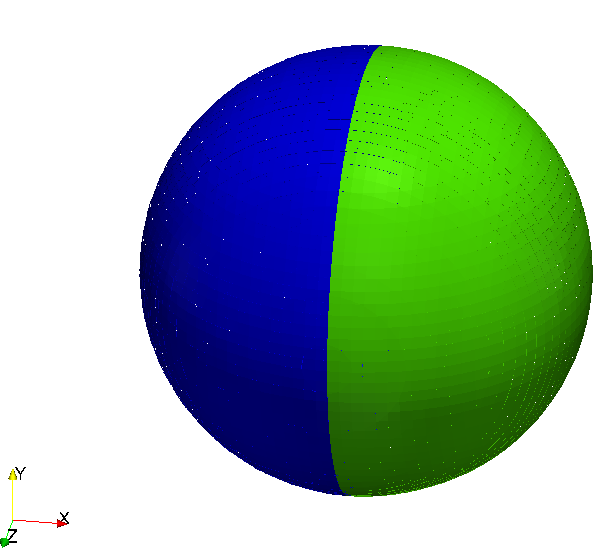
\includegraphics[width=0.94\columnwidth]{figures/rotation-hex-128-Co-05.png}
       %\label{fig:sphereFine:refined}
       \caption{Mesh with $128^3$ volumes}
   \end{subfigure}

    \caption{Visual comparison of the intial (blue) and the final (green) sphere shape
 for different densities of the \emph{rotation} test}

    \label{fig:rotation:initialFinal}
   }
\end{figure}

\subsubsection{Shear test case}

\begin{table} 
\footnotesize
\centering 
    \caption{Advection errors for the shear test case} 
    \label{tab:errors:shear} 
    \begin{tabular}{c c c c c c} 
          \toprule
          Number of volumes & $16^3$ & $32^3$ & $64^3$ & $128^3$ & \\ 
          \hline
          \hline
          Courant number &&&&& \\
          0.1   & 1.03638e-02 & 4.71128e-03 & 1.49640e-03 & 5.68667e-04 & \\ 
          0.5   & 1.11825e-02 & 5.78071e-03 & 2.59552e-03 & 1.18850e-03 & \\ 
          0.75  & 1.28960e-02 & 6.13972e-03 & 3.27130e-03 & 1.60405e-03 & \\ 
          \bottomrule
    \end{tabular}
\end{table}

\begin{figure}
   {\footnotesize
   \centering
   \begin{subfigure}[b]{0.49\textwidth}
       \centering
       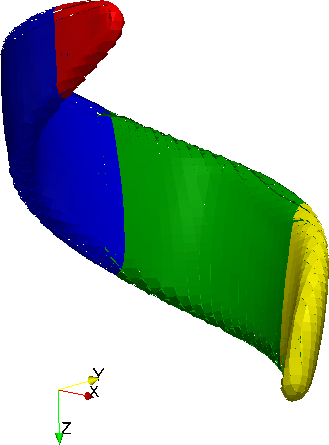
\includegraphics[width=0.8\textwidth]{figures/shear-hex-64-extreme-isometry.png}
       \caption{Extreme shear: colors mark parallel process domains} 
       \label{fig:shear:extreme}
   \end{subfigure}
   \begin{subfigure}[b]{0.49\textwidth}
       \centering
       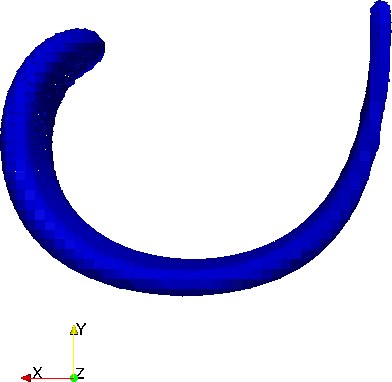
\includegraphics[width=\textwidth]{figures/shear-hex-64-extreme.png}
       \label{fig:shear:top}
       \caption{Extreme shear: projection in the direction of the Z-axis}
   \end{subfigure}
\vspace{0.5cm}

   \begin{subfigure}[b]{0.5\textwidth}
       \centering
       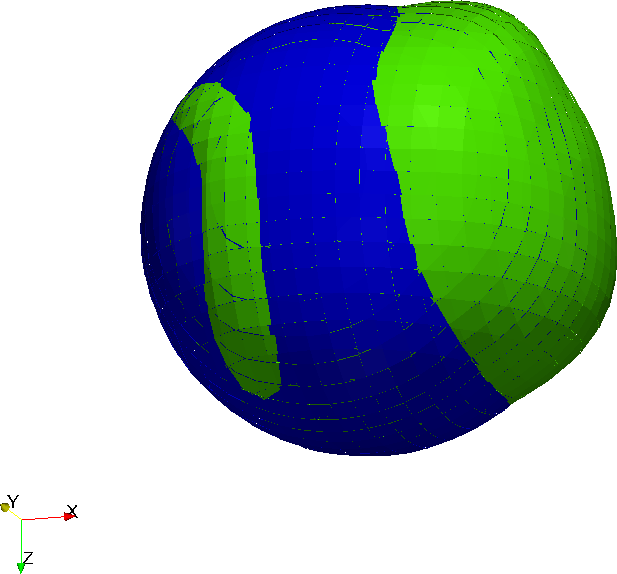
\includegraphics[width=\textwidth]{figures/shear-hex-64-comparison.png}
       \caption{Initial (blue) and the final (green) sphere shape} 
       \label{fig:shear:comparison}
   \end{subfigure}

    \caption{Shear test case on a mesh with $64^3$ volumes}
    \label{fig:shear}
   }
\end{figure}

The shear test case configuration is described by \citet{LiovicCVTNA2006} in the following way:
%
\begin{align}
    \U(\x,\,t) = 
    \left(      
			\begin{array}{l}
				\sin(2\pi y) \sin(\pi x)^2 \cos \left(\frac{\pi t}{T}\right)\\
				-\sin(2\pi x) \sin(\pi y)^2 \cos \left(\frac{\pi t}{T}\right)\\
				u_\text{max} \left(1 - \frac{r}{R}\right)^2 \left(\frac{\pi t}{T}\right)
			\end{array}
    \right)
%    U_x & = \sin(2\pi y) \sin(\pi x)^2 \cos \left(\frac{\pi t}{T}\right), \nonumber \\
%    U_y & = -\sin(2\pi x) \sin(\pi y)^2 \cos \left(\frac{\pi t}{T}\right), \\
%    U_z & = U_{max} \left(1 - \frac{r}{R}\right)^2 \left(\frac{\pi t}{T}\right).\nonumber
    \label{equation:shear-test-case}
\end{align}
%
We have used $T=3$, $u_\text{max} = 1$ and $R=0.5$ for the case settings to ensure
that the shear of the sphere will be extreme, which is visible in Figure
\ref{fig:shear:extreme}. The advection error $E_g$ of the shear test case is
shown on the Table \ref{tab:errors:shear}. The velocity field of the shear flow
test case is changing both in time and space, so the Courant number values are
computed for the maximal velocity in the flow domain for the current time step.
This Courant number value is then used to correct the time step for the next
iteration in order to maintain the prescribed fixed maximal Courant number. 

Figure \ref{fig:shear} shows the extreme state of the sphere in an imposed
shear flow, as well as the comparison between the initial and the final sphere
state for a mesh of $64^3$ volumes. The validation test cases with mesh
densities of $64^3$ and $128^3$ were run in parallel in order to validate the
computation of the volumetric phase flux across process domains for complex
flows. No differences in the results between the parallel and serial runs have 
been observed. The static parallel domain decomposition is shown in Figure
\ref{fig:shear:extreme} with different colours.

The quantitative results shown in the Table \ref{tab:errors:shear} as well as
the results shown in Figure \ref{fig:shear} present first (to the best of our
knowledge) numerically stable (mass conservative and numerically bounded)
results involving a three dimensional spatially complex and time-varying
velocity field used to advect the volume fraction with a directionally un-split
advection algorithm using a full discrete Lagrangian flow-map on an
unstructured mesh hexahedral mesh, in parallel. 

 
\subsubsection{Deformation test case}


The deformation test case, as described by
\citet{HernandezLopezPart1Advection2008}, reads 
%
\begin{align}
    \U(\x,\,t) = 
    \left( 
			\begin{array}{l}
			  2 \sin(2\pi y) \sin(\pi x)^2 \sin(2 \pi z) \cos \left(\frac{\pi t}{T}\right)\\
			  -\sin(2\pi x) \sin(\pi y)^2 \sin (2\pi z) \cos \left(\frac{\pi t}{T}\right)\\
			  -\sin(2\pi x) \sin(2 \pi y) \sin (\pi z)^2 \cos \left(\frac{\pi t}{T}\right)
			\end{array} 
    \right)
%    U_x & = 2 sin(2\pi y) sin(\pi x)^2 sin(2 \pi z) cos \left(\frac{\pi t}{T}\right), \nonumber \\
%    U_y & = -sin(2\pi x) sin(\pi y)^2 sin (2\pi z) cos \left(\frac{\pi t}{T}\right), \\
%    U_z & = -sin(2\pi x) sin(2 \pi y) sin (\pi z)^2 cos \left(\frac{\pi t}{T}\right), \nonumber
    \label{equation:deformation-test-case}
\end{align}
%
and we chose $T=3$ to ensure extreme deformation of the sphere. Table
\ref{tab:errors:deformation} shows the advection error values $E_g$ for
deformation test cases of different Courant numbers, $0.1$, $0.5$, and $0.75$,
as well as increasing mesh densities, $16^3$, $32^3$, $64^3$ and $128^3$.
Figure \ref{fig:deformation:comparison} shows a comparison between the initial
and final interface for the maximal Courant number $0.5$ and the mesh density
$128^3$, and Figure\ref{fig:deformation:extreme} shows the extreme deformation
of the sphere for the same parameter values. 

The geometrical instability present in the lower-middle part of the deformed
interface in the extreme shear state is visible in Figure
\ref{fig:deformation:extreme}. The cause of the instability lies in the fact
that the interface in this region becomes extended into a very narrow filament.
When the thickness of the layer approaches the cell size, the gradient
calculation of the Young's reconstruction method is not accurate enough to
stabilize the orientation of the interface normal. This is a common issue of
the geometrical VoF method and a detailed description is provided by
\citet{Cerne2002}. Two solutions may be applied in this case: a higher order
reconstruction and/or local dynamic AMR. A higher order reconstruction method
usually involves optimization of the interface normal orientation, which brings
additional computational cost to the overall algorithm. On the other hand, the
local dynamic AMR increases the accuracy of both the geometrical advection and
the flow solution. The \emph{locally increased mesh density } provided by local
dynamic AMR will enable the geometrical algorithm to resolve very thin
filaments, as well as the boundary layer surrounding the interface, while
keeping a \emph{low overall number of cells} in the mesh, thus increasing the
overall efficiency of the solution. 

\begin{table} 
\footnotesize
\centering 
\caption{Advection errors of deformation test case} 
\label{tab:errors:deformation} 
    \begin{tabular}{c c c c c c} 
          \toprule
          Number of volumes & $16^3$ & $32^3$ & $64^3$ & $128^3$ & \\ 
          \hline
          \hline
          Courant number &&&&& \\
          0.1   & 1.34430e-02 & 7.776114e-03 & 1.53454e-03 & 8.09107e-04 & \\  
          0.5   & 1.48808e-02 & 8.157570e-03 & 2.53035e-03 & 1.30304e-03 & \\  
          0.75  & 1.58007e-02 & 8.978900e-03 & 3.17220e-03 & 1.58943e-03 & \\ 
          \bottomrule
    \end{tabular}
\end{table}

\begin{figure}
   {\footnotesize
   \centering
   \begin{subfigure}[b]{0.49\textwidth}
       \centering
       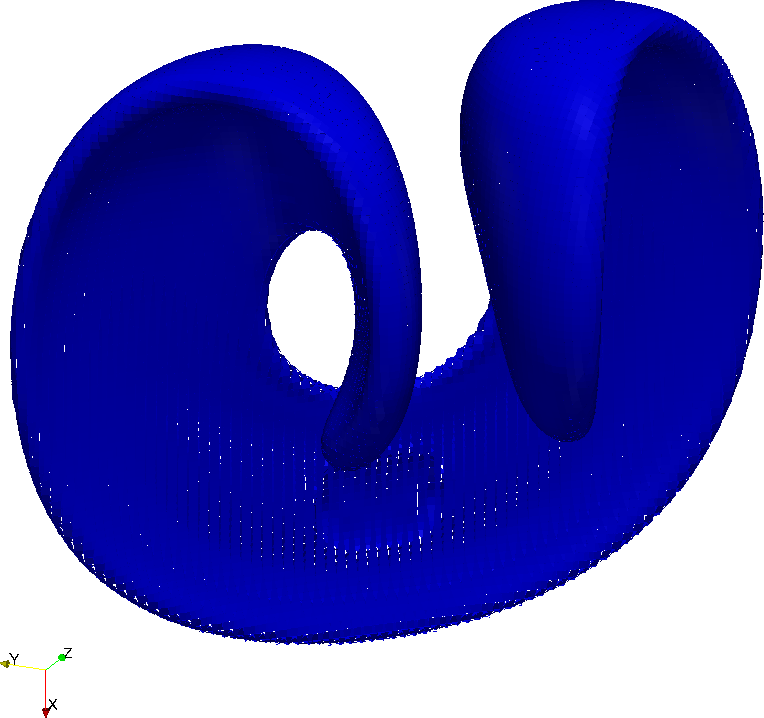
\includegraphics[width=\textwidth]{figures/deformation-hex-128-Co-05-extreme.png}
       \caption{Extreme deformation of a sphere} 
       \label{fig:deformation:extreme}
   \end{subfigure}
   \begin{subfigure}[b]{0.5\textwidth}
       \centering
       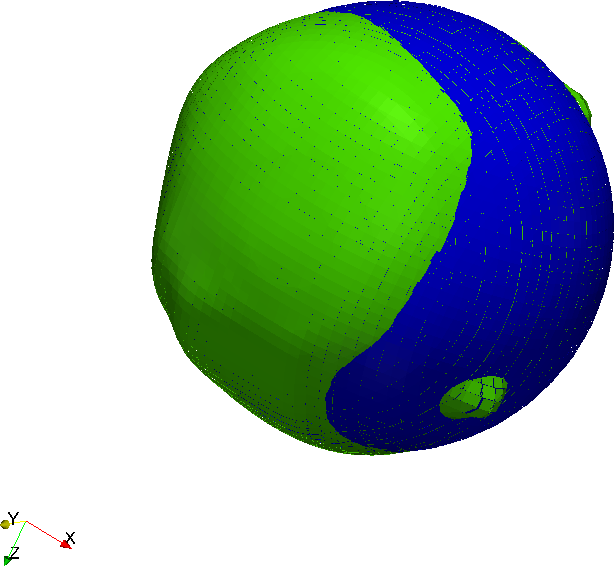
\includegraphics[width=\textwidth]{figures/deformation-hex-128-Co-05-comparison.png}
       \caption{Initial (blue) and the final (green) sphere shape} 
       \label{fig:deformation:comparison}
   \end{subfigure}

       \caption{Deformation test case on a mesh with $128^3$ volumes}

    \label{fig:deformation}
   }
\end{figure}

\subsection{Results using local adaptive AMR}

\begin{figure}
   {\footnotesize
   \centering
   \begin{subfigure}[b]{0.43\textwidth}
       \centering
       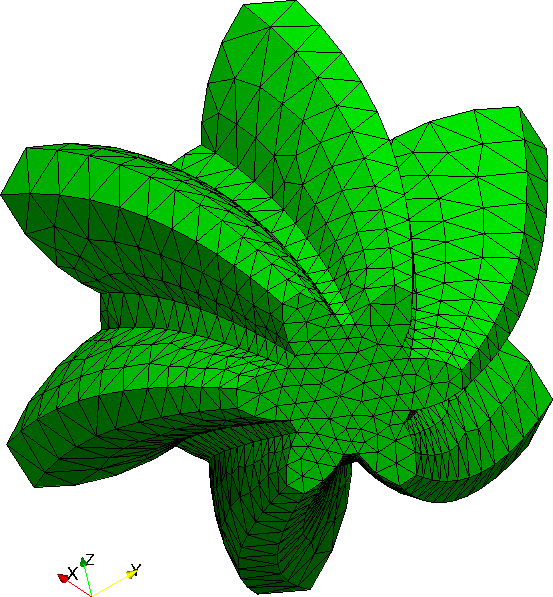
\includegraphics[width=\textwidth]{figures/helical-inputmesh.png}
       \caption{Input mesh (exact interface)} 
       \label{fig:helical:input}
   \end{subfigure}
   \quad
   \begin{subfigure}[b]{0.43\textwidth}
       \centering
       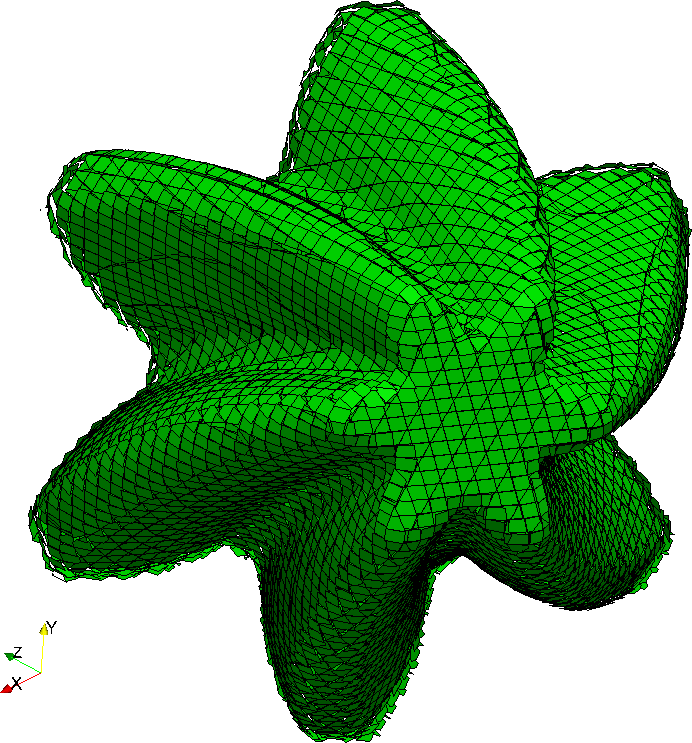
\includegraphics[width=\textwidth]{figures/helical-level4-front.png}
       \caption{Reconstructed interface: front view}
       \label{fig:helical:final-front}
   \end{subfigure}
\vspace{0.5cm}

   \begin{subfigure}[b]{0.43\textwidth}
       \centering
       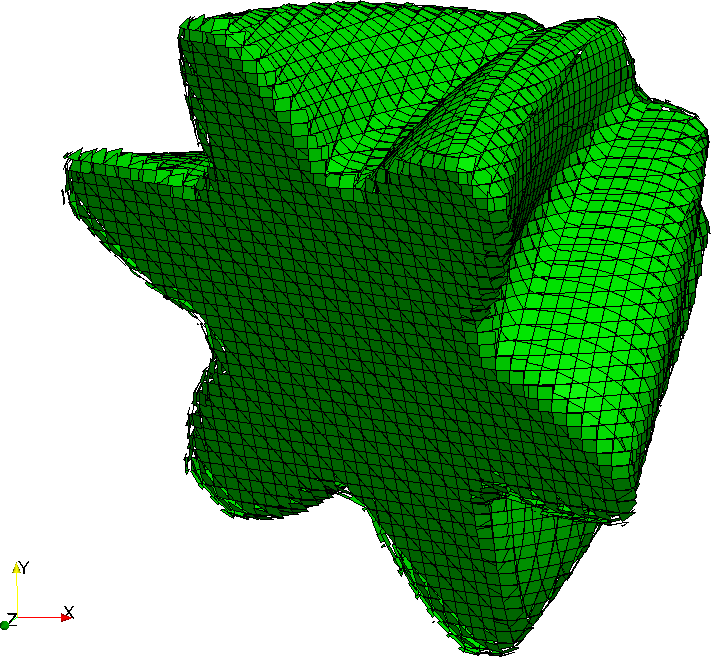
\includegraphics[width=\textwidth]{figures/helical-level4-back.png}
       \caption{Reconstructed interface: back view}
       \label{fig:helical:final-back}
   \end{subfigure}
   \quad
   \begin{subfigure}[b]{0.43\textwidth}
       \centering
       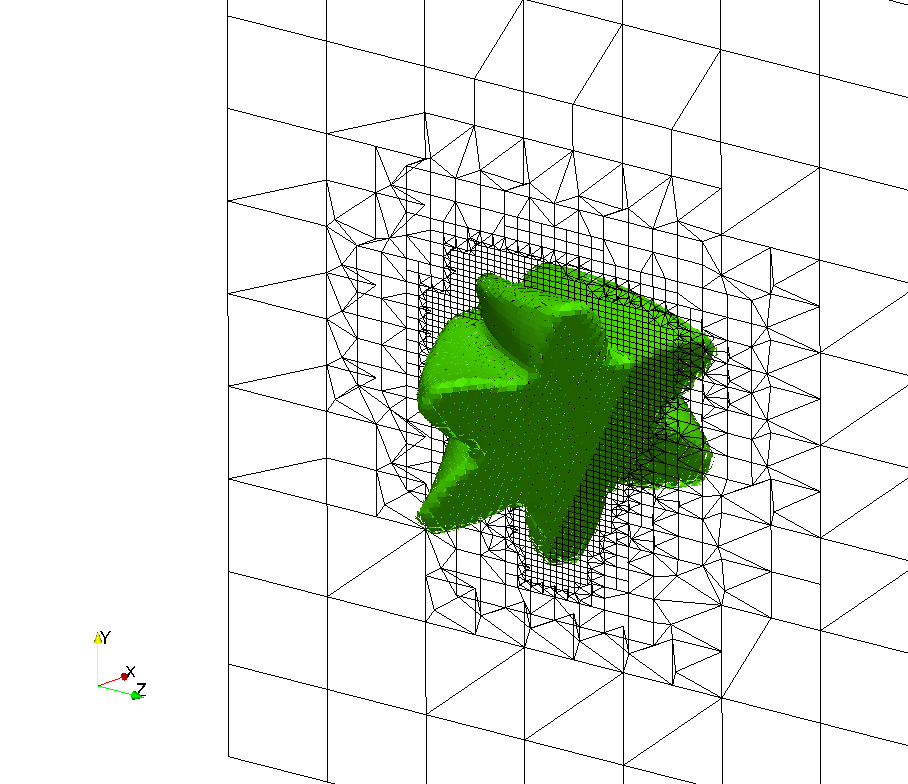
\includegraphics[width=\textwidth]{figures/refined-green-black.png}
       \caption{Background AMR refined mesh (wireframe) and reconstructed interface} 
       \label{fig:helical:final-background}
   \end{subfigure}

       \caption{Illustration of capability to reconstruct complex interface geometries: Interface 
         reconstruction for a helical gear geometry using local dynamic AMR}

    \label{fig:helical}
   }
\end{figure}

\subsubsection{Reconstruction}

To emphasize the advantages of basing our developments on an arbitrary
unstructured mesh, we have chosen a reconstruction verification case involving
a complex geometry. Arbitrarily, a geometry has been chosen consisting of a head 
part of a helical transmission gear for which the mesh was automatically generated. 
Clearly, this choice of the interface geometry is artificial, however it shows that 
arbitrary complexity of the interface reconstruction can be fully resolved with very 
little computational overhead using local dynamic AMR on unstructured hexahedral meshes, 
even with a geometrically first order convergent reconstruction algorithm.

Figure \ref{fig:helical:input} shows the prescribed interface in the form of a
helical gear (input mesh). The interface reconstructed with a refinement
level of $4$ is shown in the front view in Figure \ref{fig:helical:final-front}
and from the back view in Figure \ref{fig:helical:final-back}. The background mesh
of together with the refinement layers are visible in Figure
\ref{fig:helical:final-background}. Note that the initial mesh is very coarse;
the length scale of a cell is in the order of magnitude of the width of the
gear. 

Table \ref{tab:amr:reconstruction} contains the volume of symmetric difference
error $E_{vsd}$, order of error convergence, as well as normalized CPU time
and the normalized number of interface polygons with increasing level of mesh
refinement. The small order of convergence observed initially for the refinement 
level $1$ comes from the fact that the interface is severly under-resolved on the
initial very coarse  mesh. Once the local refinement reaches the cell length
scale that is enough to sufficiently resolve the curvature of the interface,
the convergence of the error increases significantly, which is expected for the
geometrically first order convergent Youngs reconstruction algorithm. With
further local mesh refinement the order of convergence of the $E_{vsd}$ error
stabilizes. 

The CPU time increases almost linearly with the increase in the number of
interface polygons, thus defining the overall reconstruction algorithm linear
in complexity $O(N_{polygons})$. This linear relationship is visualized in
Figure \ref{fig:reconstruction-cputime} in the form of a diagram.

\begin{table} 
\footnotesize
\centering 
\caption{Reconstruction data with local dynamic AMR} 
\label{tab:amr:reconstruction} 
    \begin{tabular}{l c c c c c } 
          \toprule
          Refinement level & 0 & 1 & 2 & 3 & 4\\ 
          \hline
          \hline
          %&&&&&&&& \\
          $E_{vsd}$                             & 5.36139e-06 & 3.79479e-06 & 1.37713e-06 & 3.85176e-07 & 1.27413e-07 \\  
          $E_{vsd}$ order of convergence        & n/a & 0.49 & 1.46 & 1.83  & 1.59 \\  
          Normalized number of polygons         & 1 & 3.81 & 16 & 65.35  & 315 \\ 
          Normalized CPU time                   & 1 & 1.17 & 2 & 6 & 22.67 \\ 
          \bottomrule
    \end{tabular}
\end{table}

%\begin{figure}
%    \footnotesize
%    \centering
%     \begin{tikzpicture}[]
%         \begin{loglogaxis}[
%         width=0.5\textwidth,
%         xlabel={Normalized number of interface polygons},
%         grid=both,
%         ylabel={Normalized CPU time},
%             label style={font=\footnotesize}, tick label style={font=\footnotesize},
%             y label style={at={(0.1,0.5)}}, x label style={at={(0.5,0.05)}}
%         ],
%         \addplot[color=black, mark=x] file {./figures/refinement-relative-diagram.dat};
%         \end{loglogaxis}
%     \end{tikzpicture}
%     \caption{Linear dependency of the CPU time with respect to the number of interface polygons}
%     \label{fig:reconstruction-cputime}
%\end{figure}
\begin{figure}
	\centering
		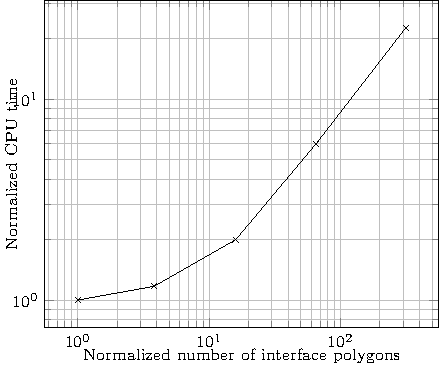
\includegraphics{./MaricMarschallBothe-voFoamAlgorithm-figure4.pdf}
     \caption{Linear dependency of the CPU time with respect to the number of interface polygons}
     \label{fig:reconstruction-cputime}
\end{figure}

\subsubsection{Advection}

In \citep*{MaricVoFoamMapping2013} we have presented the
results for the shear test case together with local dynamic AMR to verify the
geometrical mapping algorithm. Table \ref{tab:amr:shear} holds an excerpt of
the solution results for this test case. The results of the shear advection
executed together with the local dynamic AMR on an initial mesh of $16^3$
volumes are consistent with the results obtained for the corresponding
uniformly refined meshes with densities defined by the finest refinement level.
The normalized CPU time with respect to the corresponding uniform shear test
case shows the benefit of local dynamic AMR when it comes to the computational
cost. To obtain the magnitude of the volume of symmetric error $E_{vsd}$
corresponding to the mesh of $128^3$ volumes (refinement level 3), only 58\% of
the CPU time is required. Further speedup is to be achieved by refactoring and
optimization of the geometrical library. Figure \ref{fig:amr:rotation} shows the
final result of the rotation test case with local dynamic AMR (level 2
refinement).

\begin{table} 
\footnotesize
\centering 
\caption{Shear case data with local dynamic AMR} 
\label{tab:amr:shear} 
    \begin{tabular}{l c c c} 
          \toprule
          Refinement level & 1 & 2 & 3 \\ 
          \hline
          \hline
          %&&&&&&&& \\
          $E_{vsd}$                             & 5.8131E-003 & 2.7268E-003 & 1.11965E-003 \\  
          $E_{vsd}$ order of convergence        & 0.94 & 1.09 & 1.28 \\  
          Normalized CPU time                   & 0.83  & 0.71 &  0.58 \\ 
          \bottomrule
    \end{tabular}
\end{table}

\begin{figure}
    \footnotesize
    \centering
     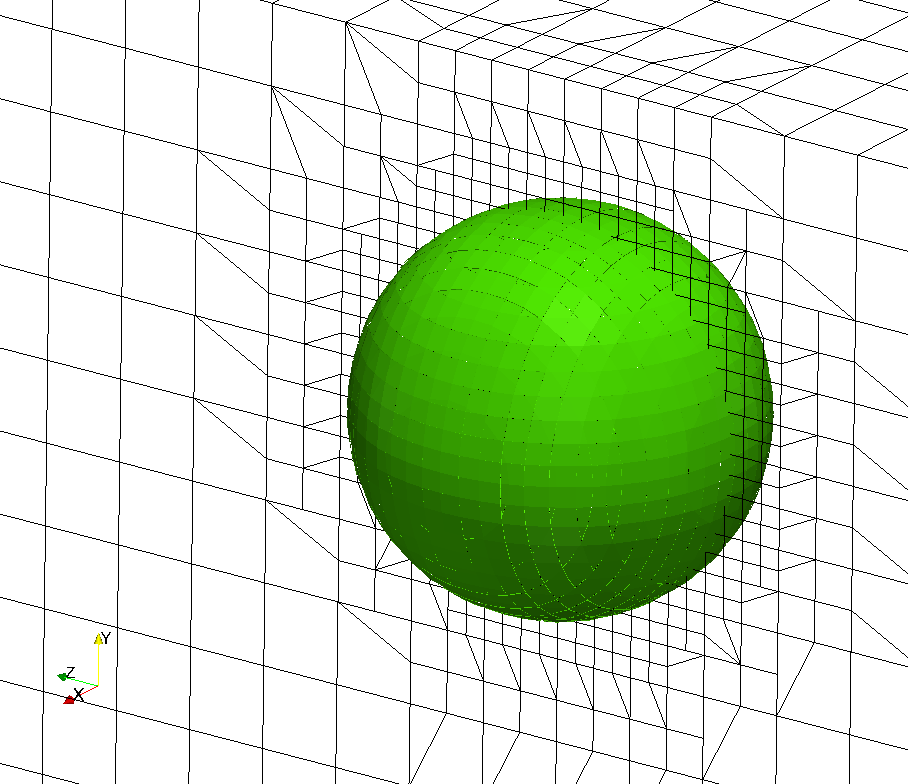
\includegraphics[width=0.5\textwidth]{figures/rotation-refined-green-black.png}
     \caption{Final sphere shape for a rotation case using local dynamic AMR with level 2 refinement}
     \label{fig:amr:rotation}
\end{figure}
